\documentclass[..\EOYR.tex]{subfiles}

\begin{document}

\section{Modelling the Gulf Stream}
\label{SEC:ModellingGulfStream}

As more scientists seek to understand ocean dynamics, more models are made and used by different researchers to simulate different processes. There are many models in use today, all with different configurations and settings. This can lead to contrasting outcomes and debate over which choice of model or model settings yields the most accurate results.

\subsection{Model Resolution}
\label{SSEC:ModelResolution}

	Along with differing numerical schemes or boundary conditions, etc. there are also many different model resolutions available. These range from coarse 1$\degree$ models, which resolve to a scale of $\approx$ 100km, to higher resolution 0.25$\degree$ models, which resolve to a scale of $\approx$ 25km, all with varying numbers of vertical levels. It is well established \citep{Scaife2011a}\citep{Hurlburt2008} that a higher resolution ocean model tends to produce a more accurately resolved Gulf Stream. This is in part due to the small scale processes, mentioned previously, which contribute to the ocean circulation, but are not resolved in the coarser models. Unfortunately higher resolution models require additional processing power and thus additional costs. This means that the high resolutions required to resolve a realistic Gulf Stream will not be widely used for some time. Hence, the aim is to find a way to represent an accurate Gulf Stream in the lower resolution models by understanding the reasons behind it.

\subsection{Vertical Coordinate System}
\label{SSEC:VerticalCoordinates}

	One of the main variabilities between different models is the handling of the vertical coordinate system. The way in which the model splits the depth of the ocean into 'levels' can have a large impact on the way the bathymetry is represented. As previously discussed, this bathymetric representation can have large impacts on the dynamics within the model. The importance and significance of the bathymetric roughness has already been discussed in this review so it is now necessary to discuss the different ways to represent this.
    \par
The main coordinate systems in use are the z-coordinate system which stays true to a cartesian system of coordinates, consisting of rectangular 'blocks', which create a staircase effect when representing slopes. These z-coordinate systems can also be implemented with 'partial cells' whereby some of the cells are cut into smaller cells to 'smooth out' and more closely represent the shape of the slopes. Thre are also s- (or sigma-) coordinates which follow the shape of the terrain. The depth at any point is divided by the number of levels to create a consistent number of cells at all points of different thickness. These different approaches can also be combined to form hybrid coordinate systems. See Figure \ref{FIG:Coords} for an illustration of some of the possible vertical coordinate systems available in the NEMO model.

\begin{figure}[t]
  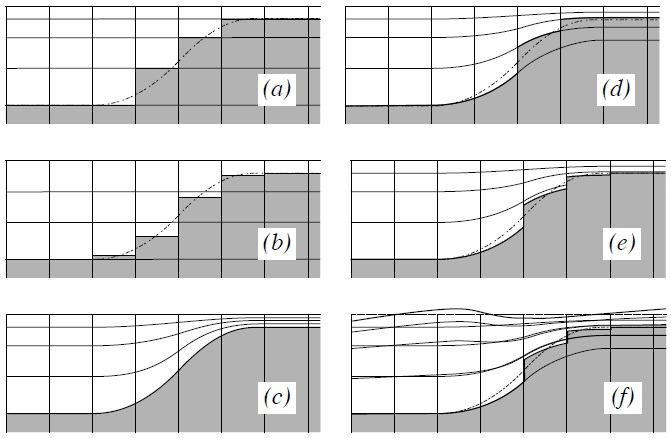
\includegraphics[width=\linewidth]{Figures/NEMOP58.jpg}
  \caption{An illustration of different veritcal coordinate systems available in NEMO. \citep{Madec2011}. (a) z-coordinate, (b) z-coordinate with partial cells, (c) s-coordinate, (d) hybrid s-z coordinate, (e) hybrid s-z coordinate with partial cell, (f) shows (e) with a non-linear free surface (which can be used with any coordinate system).}
  \label{FIG:Coords}
\end{figure}

The main difficulty in comparing different vertical coordinate systems lies in the availability of a 'control' case for the comparison. With the wide selection of models available to researchers, it is not only the vertical coordinate system which differs but also the numerical schemes being used to resolve various processes. This could lead to false similarities or differences and cause incorrect conclusions. \citep{Ezer2016b} was able to compare results from z-coordinate models and s-coordinate models while minimalising any other differnces between the models. Although the z-coordinate models are capable of producing an accurate Gulf Stream at hight resolutions, the s-coordinate models provided a more accurate representation when restricted with coarser models. However, as \citep{Ezer2016b} noted in the comparison, partial and shaved cells (whereby corners of the cells are 'shaved' off to smooth out slopes) were not used in any of these models.



\end{document}
